\section{Future Land Use}

\noindent \hl{[do more to fully introduce this section]}\\

\noindent Maps on the following pages are the proposed future land use (FLU) maps for Bloomfield's entire zoning jurisdiction. They should guide all land use and development decisions over the next ten years. Should the Bloomfield Planning Commission and the City Council choose to make policy decisions that are not reflected on the FLU map, then the FLU map must be amended to reflect the change in policies.

\thispagestyle{empty}
\begin{landscape}
    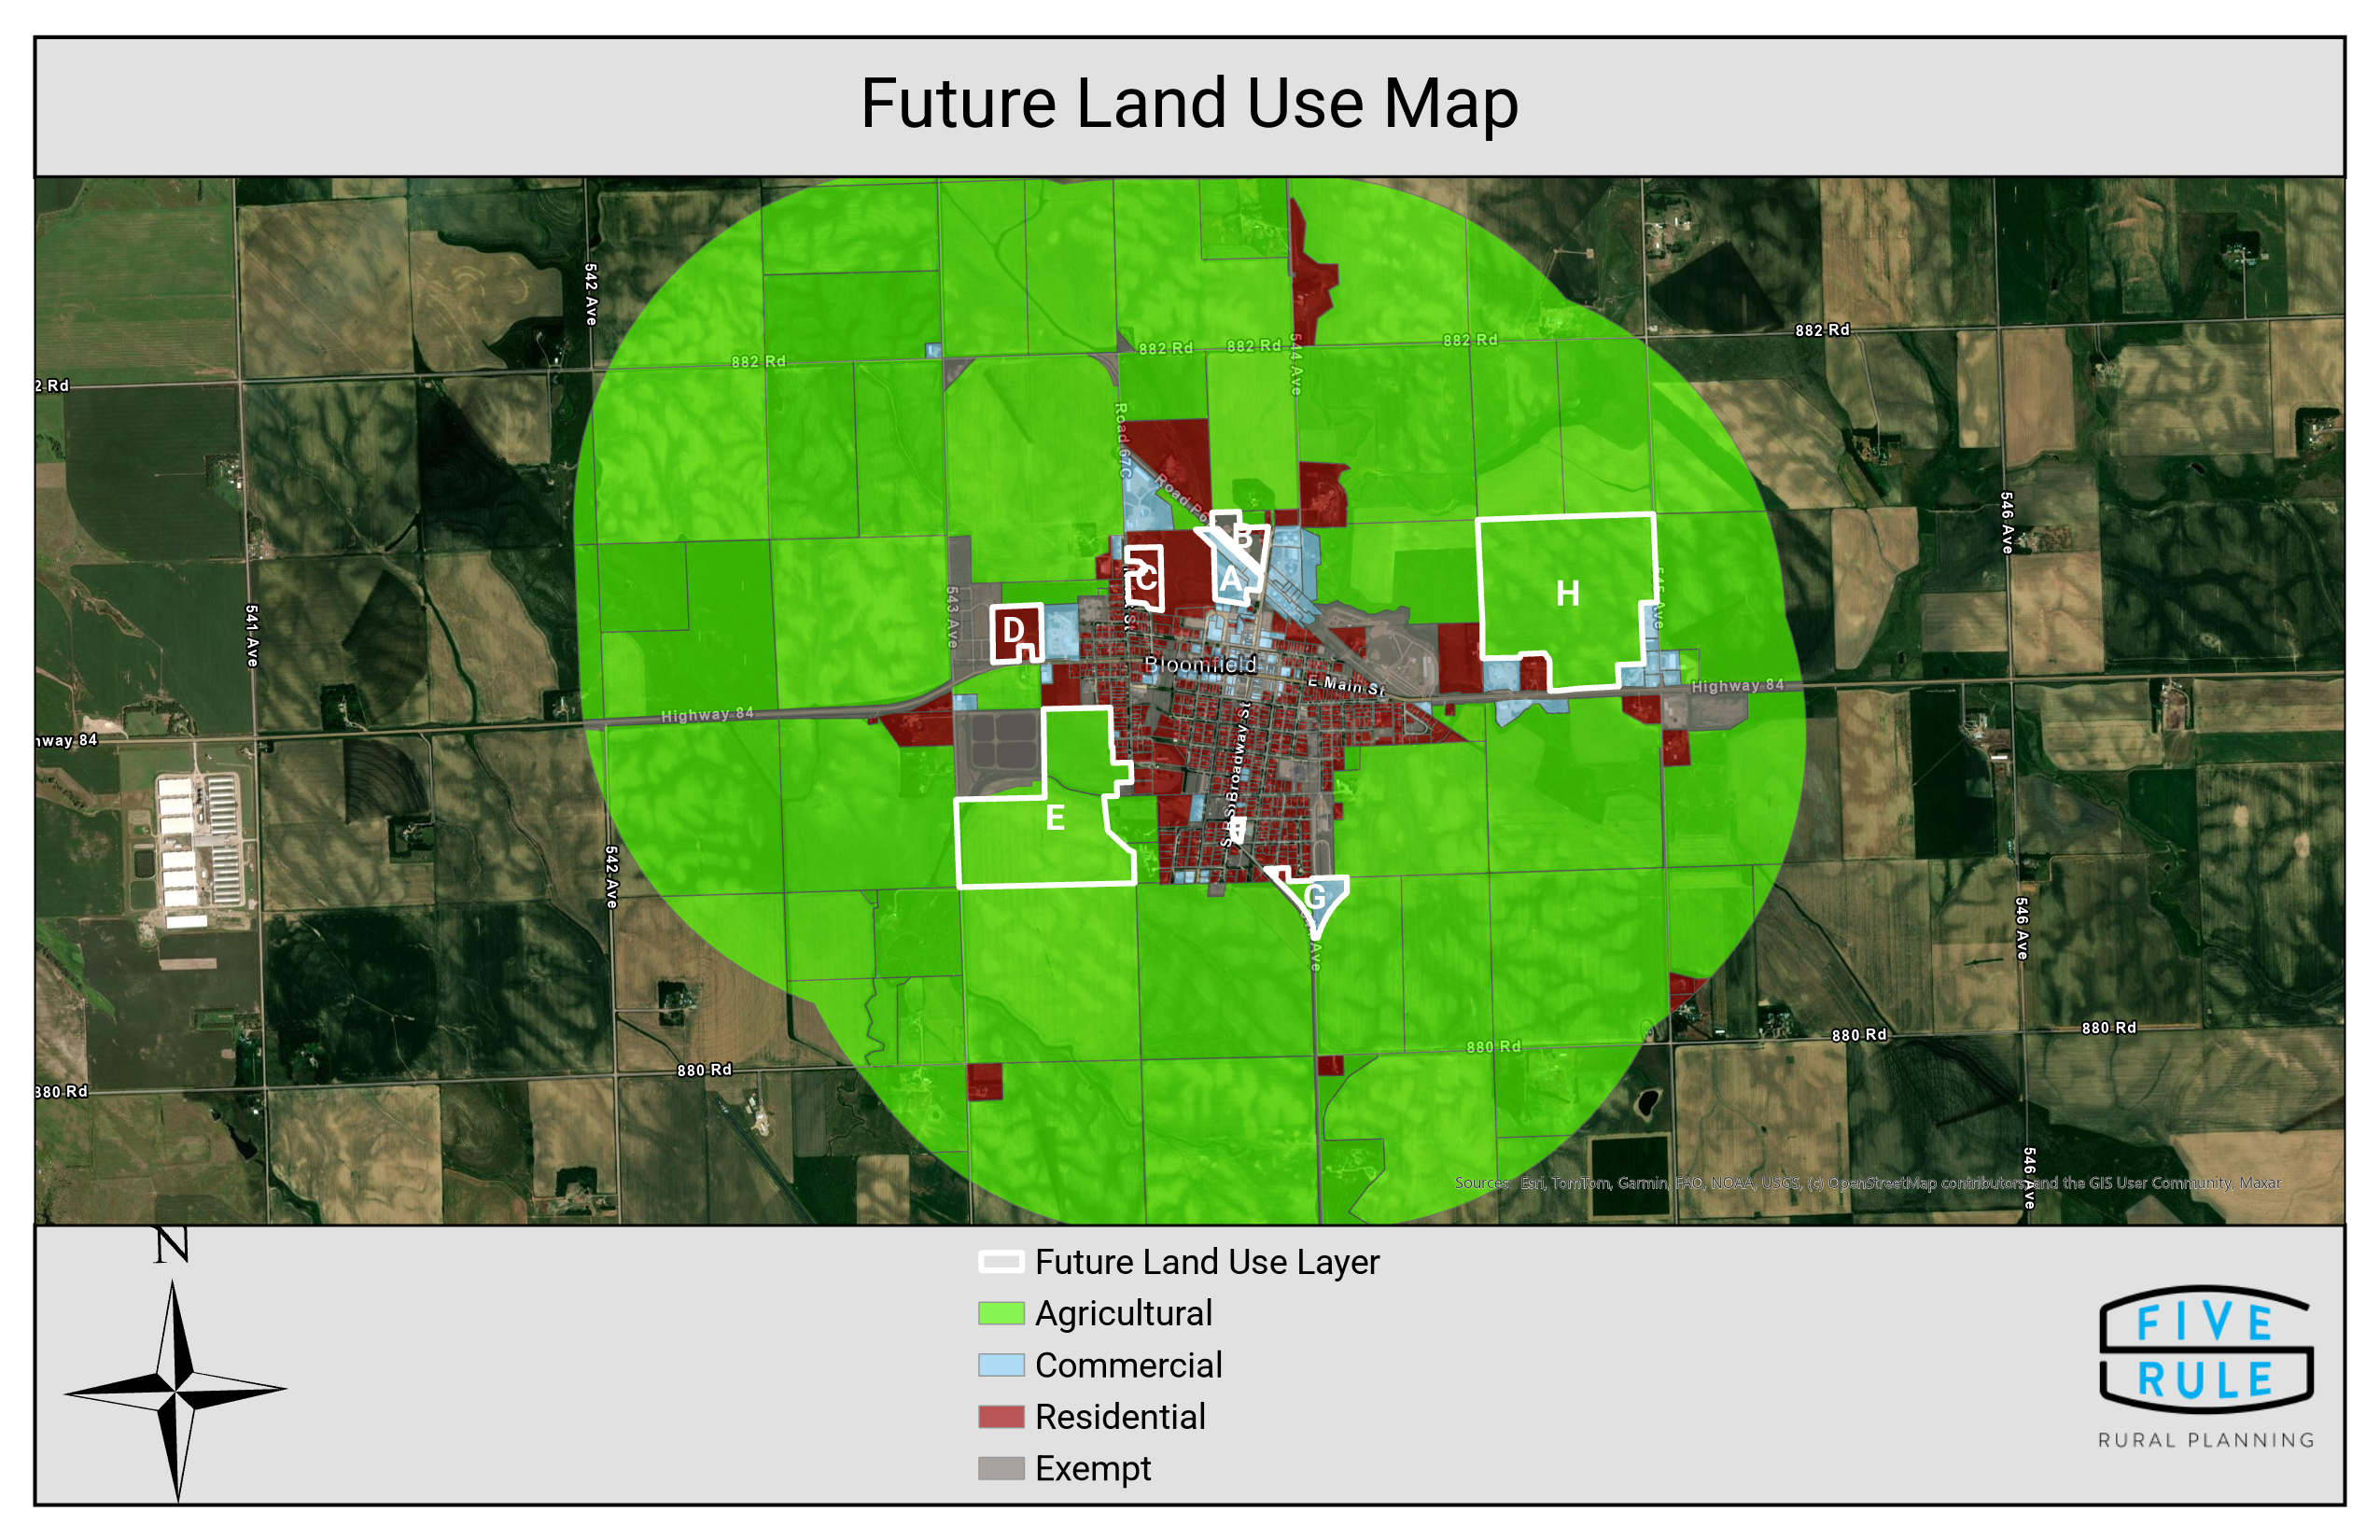
\includepdf[angle = 90]{maps/flu_all.pdf}
\end{landscape}

\pagebreak
\thispagestyle{empty}
\begin{landscape}
    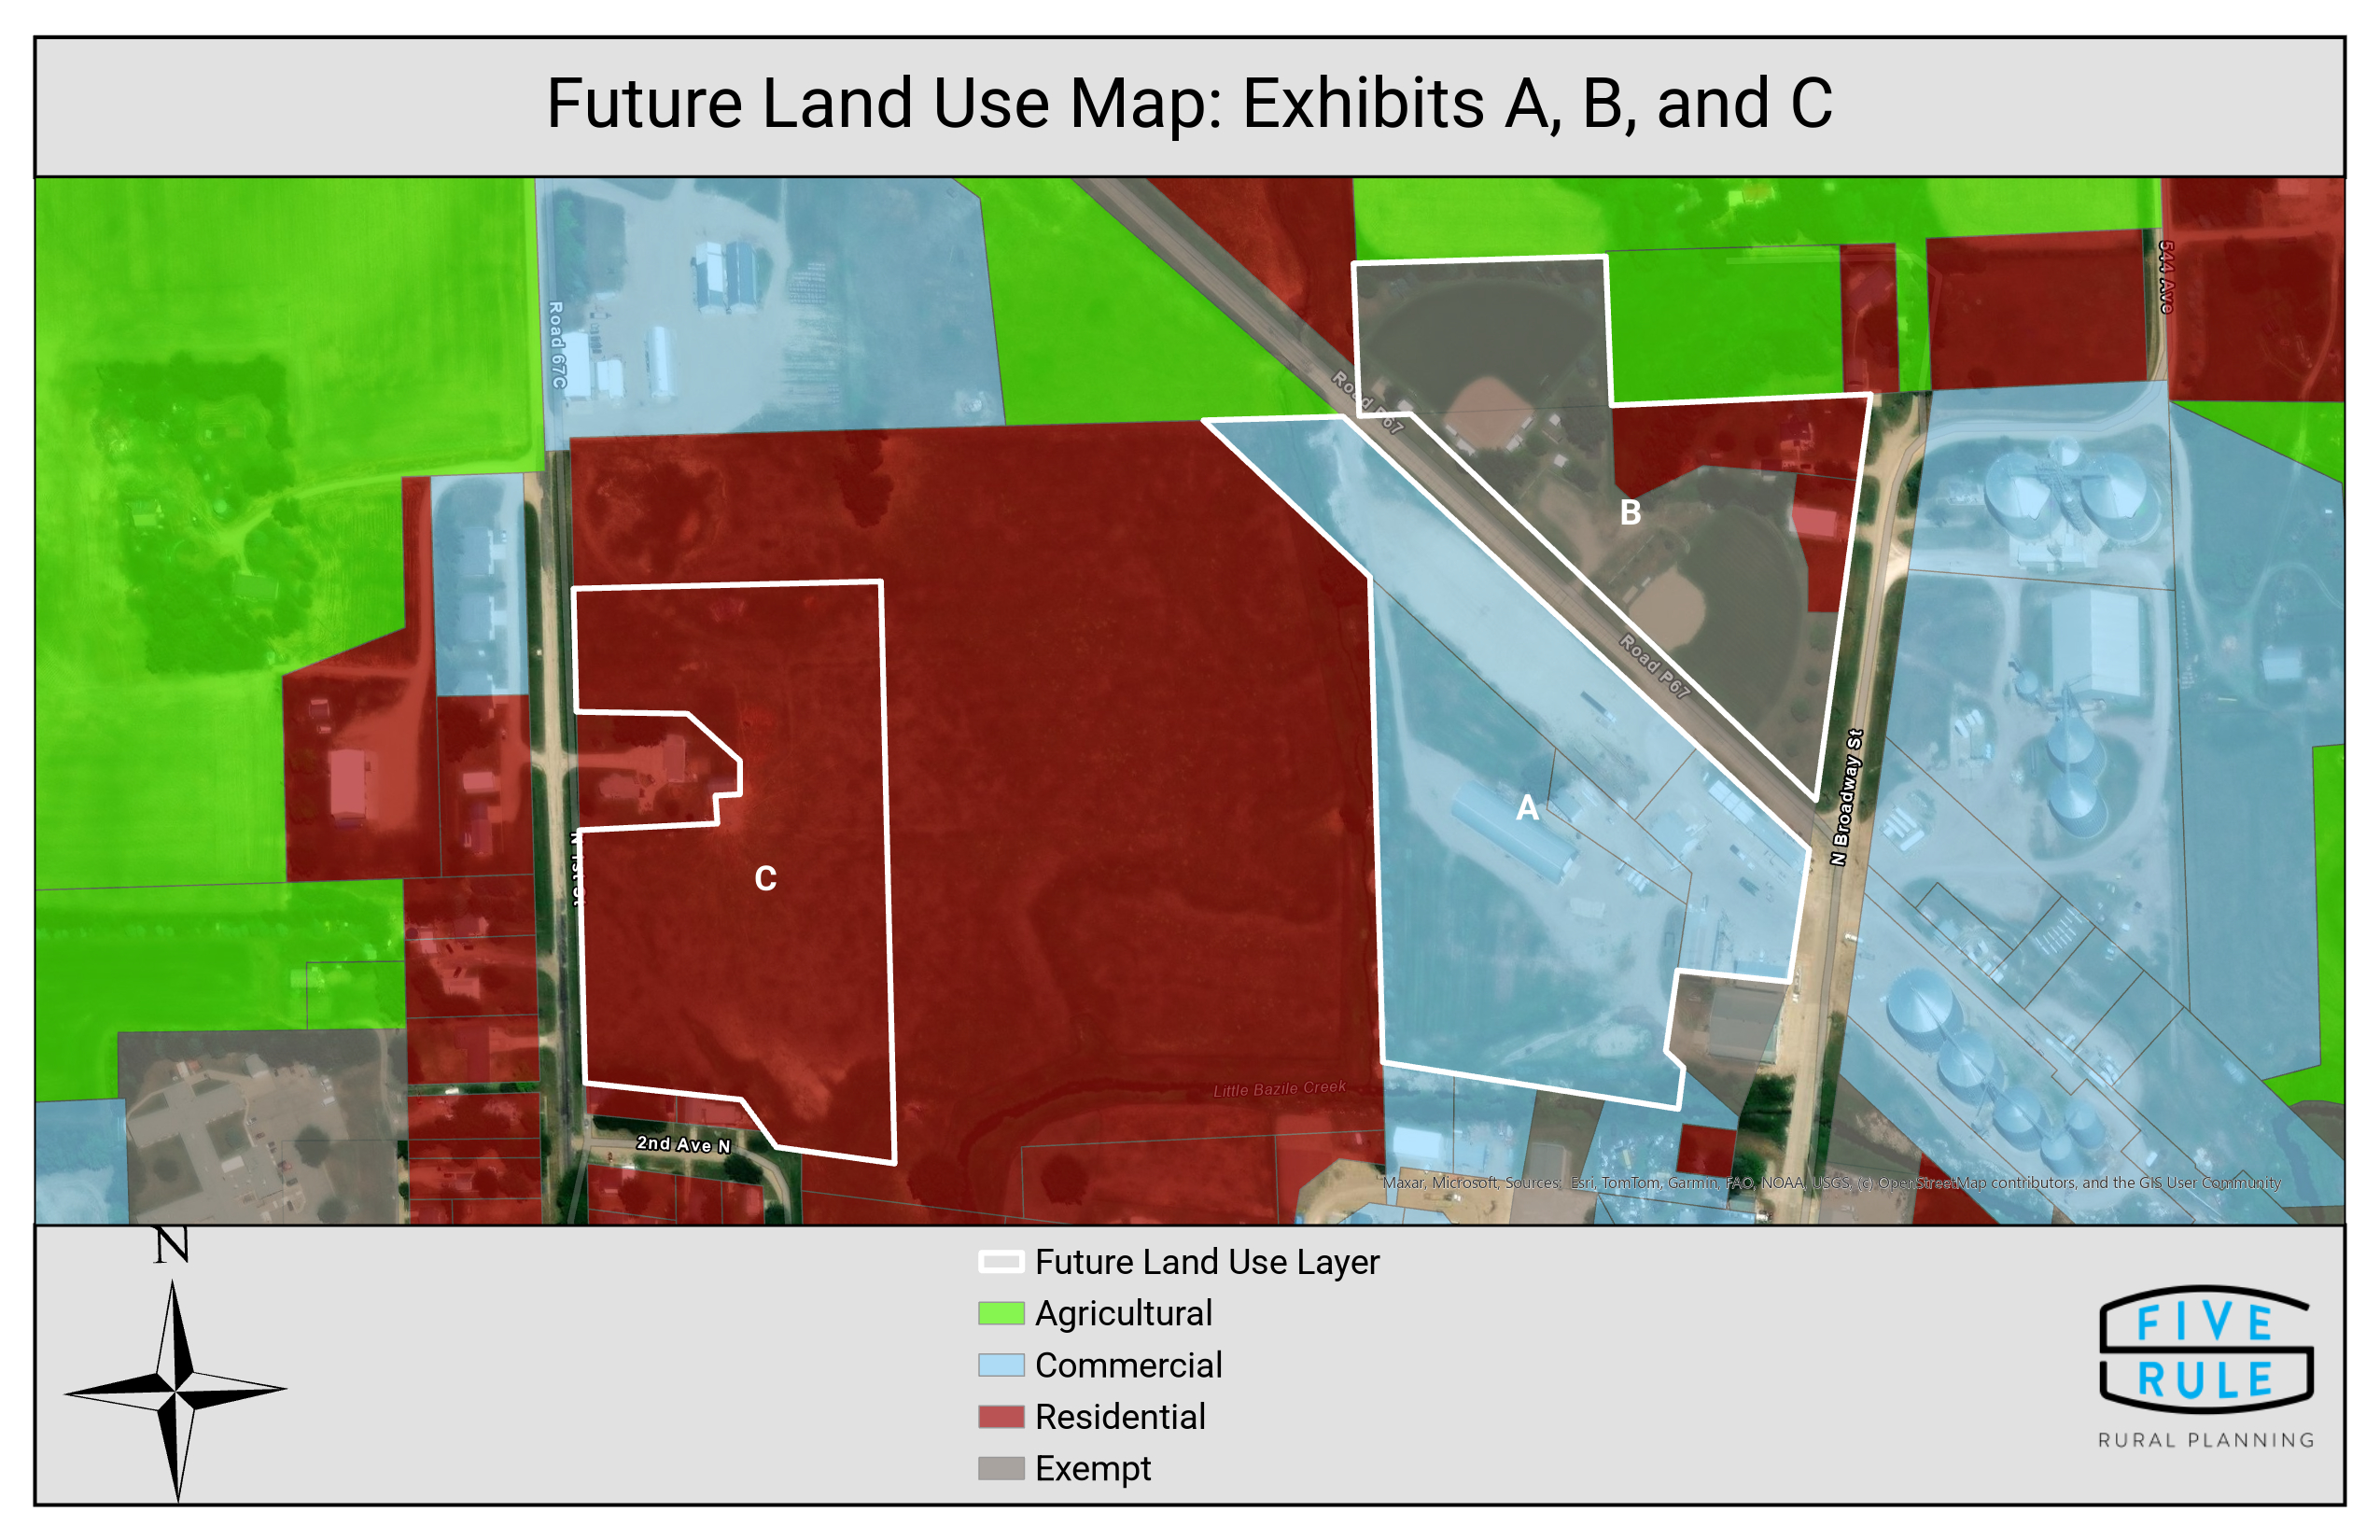
\includepdf[angle = 90]{maps/flu_abc.pdf}
\end{landscape}

\pagebreak
\thispagestyle{empty}
\begin{landscape}
    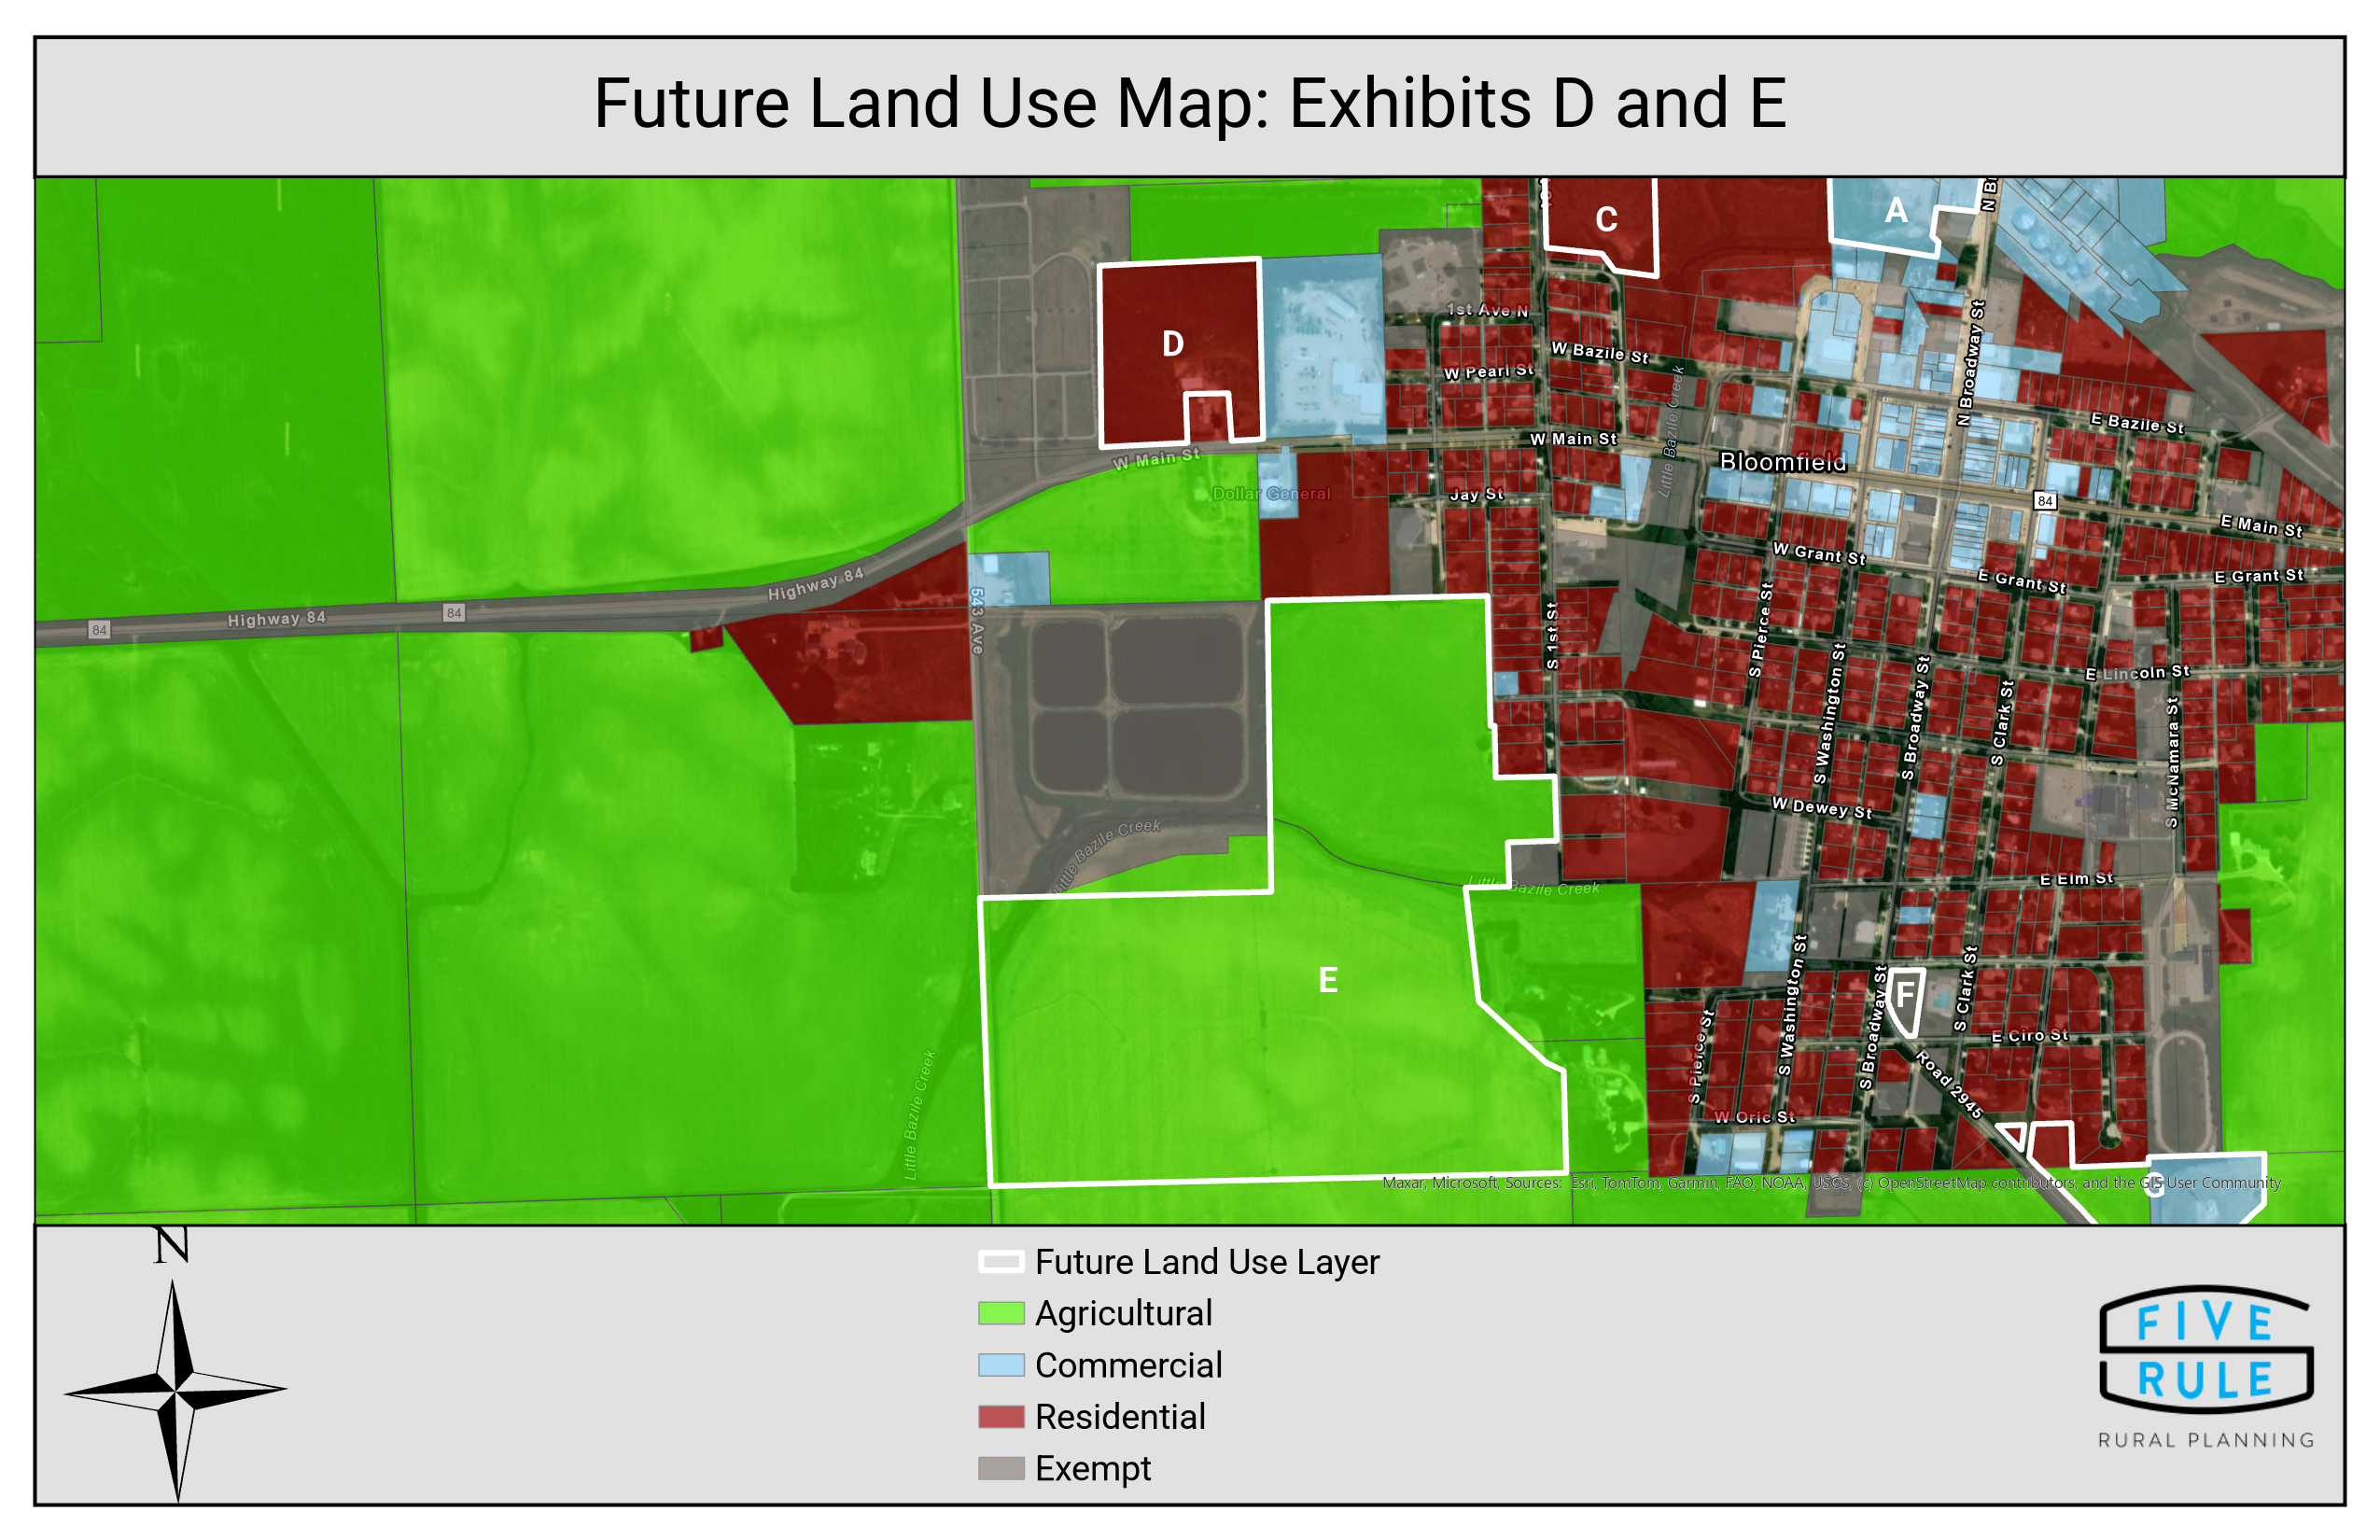
\includepdf[angle = 90]{maps/flu_de.pdf}
\end{landscape}

\pagebreak
\thispagestyle{empty}
\begin{landscape}
    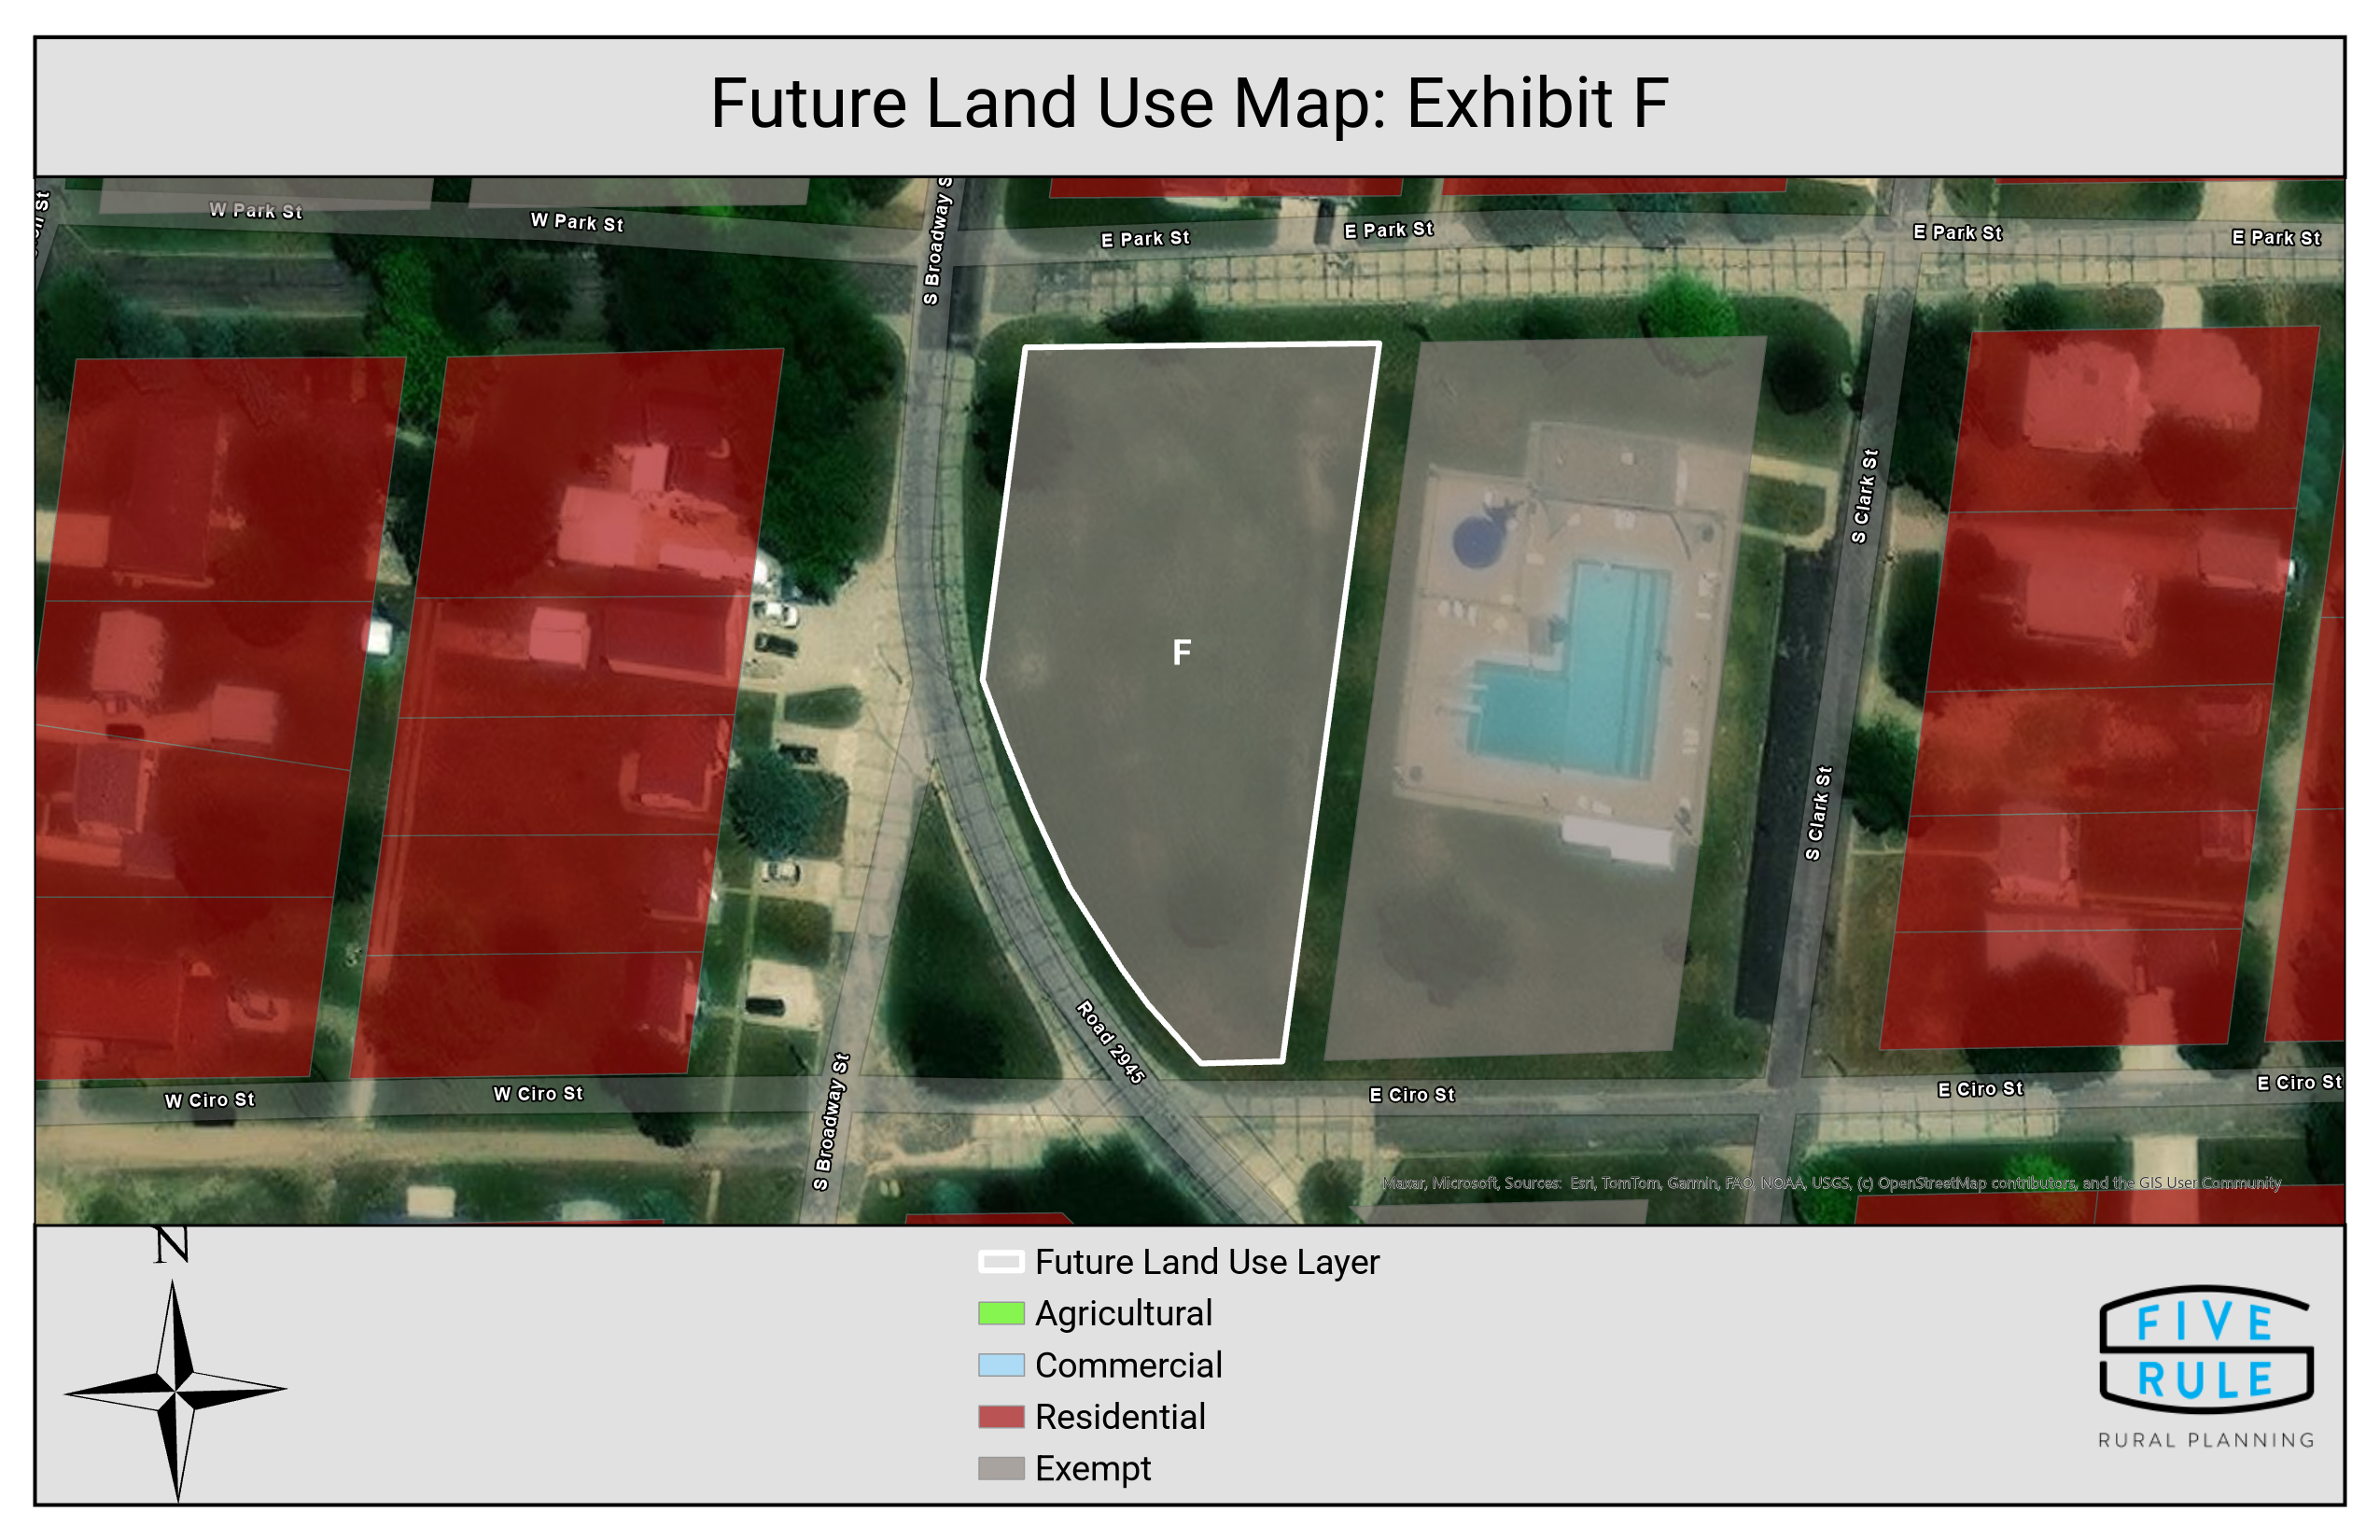
\includepdf[angle = 90]{maps/flu_f.pdf}
\end{landscape}

\pagebreak
\thispagestyle{empty}
\begin{landscape}
    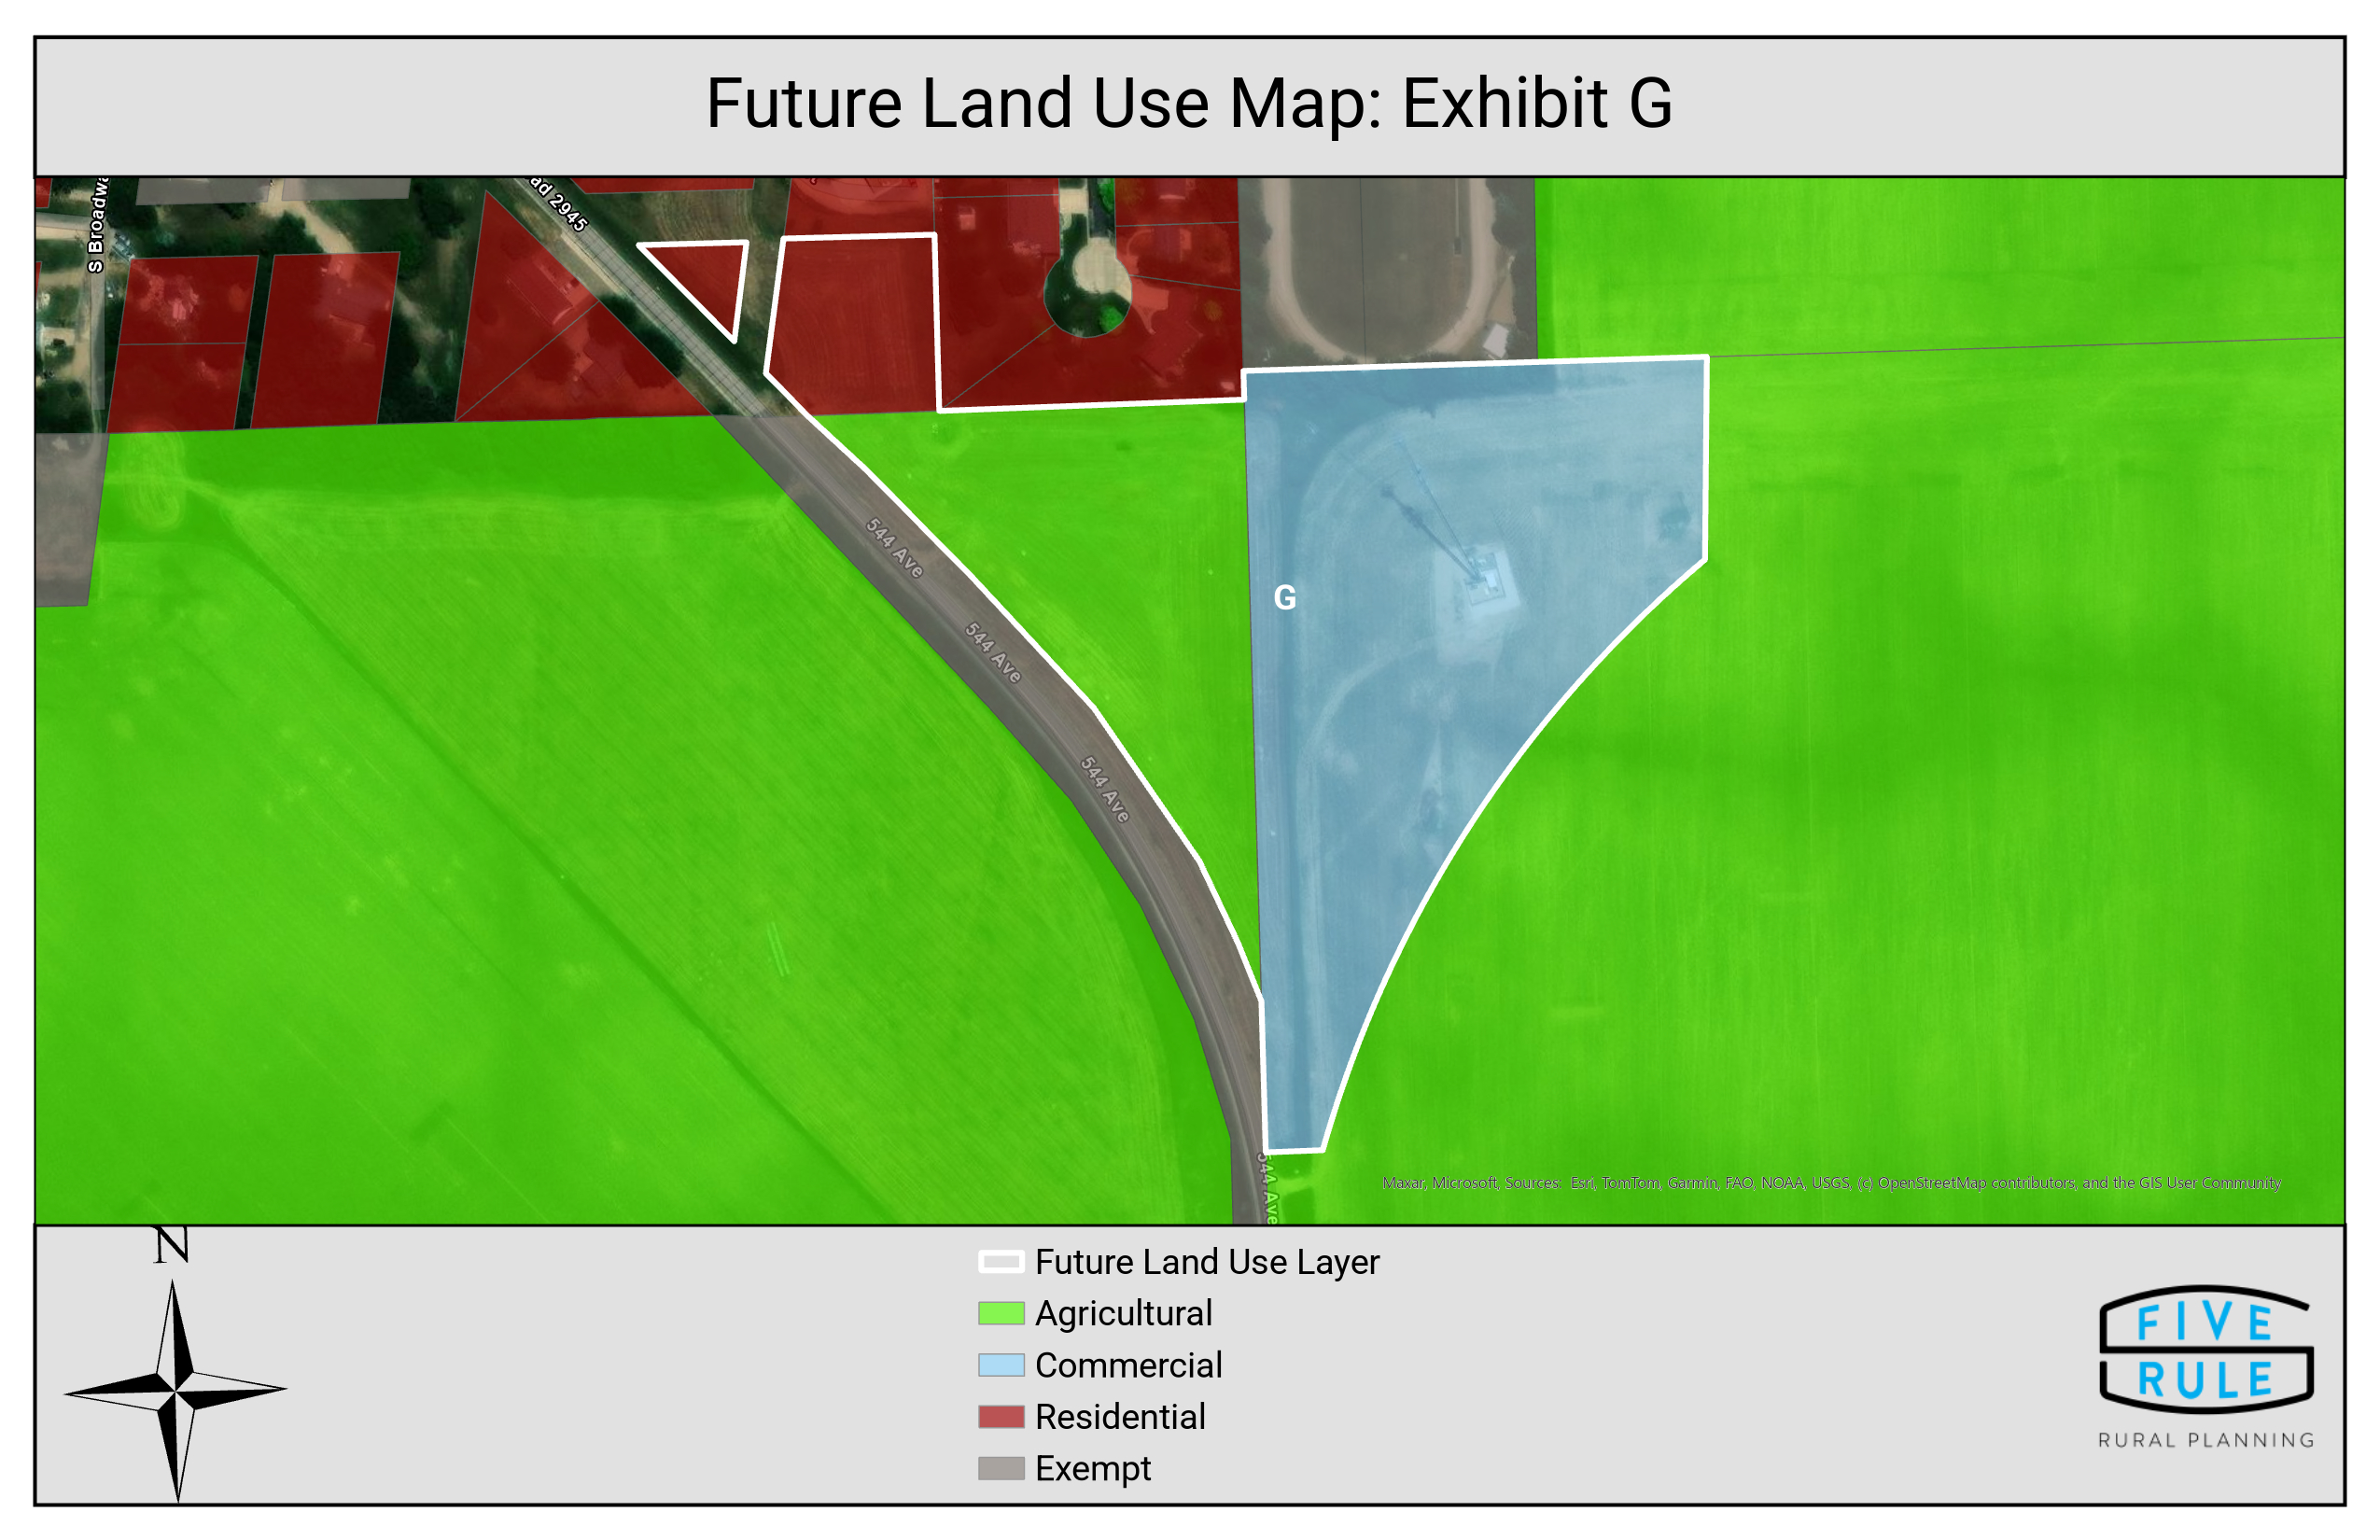
\includepdf[angle = 90]{maps/flu_g.pdf}
\end{landscape}

\pagebreak
\thispagestyle{empty}
\begin{landscape}
    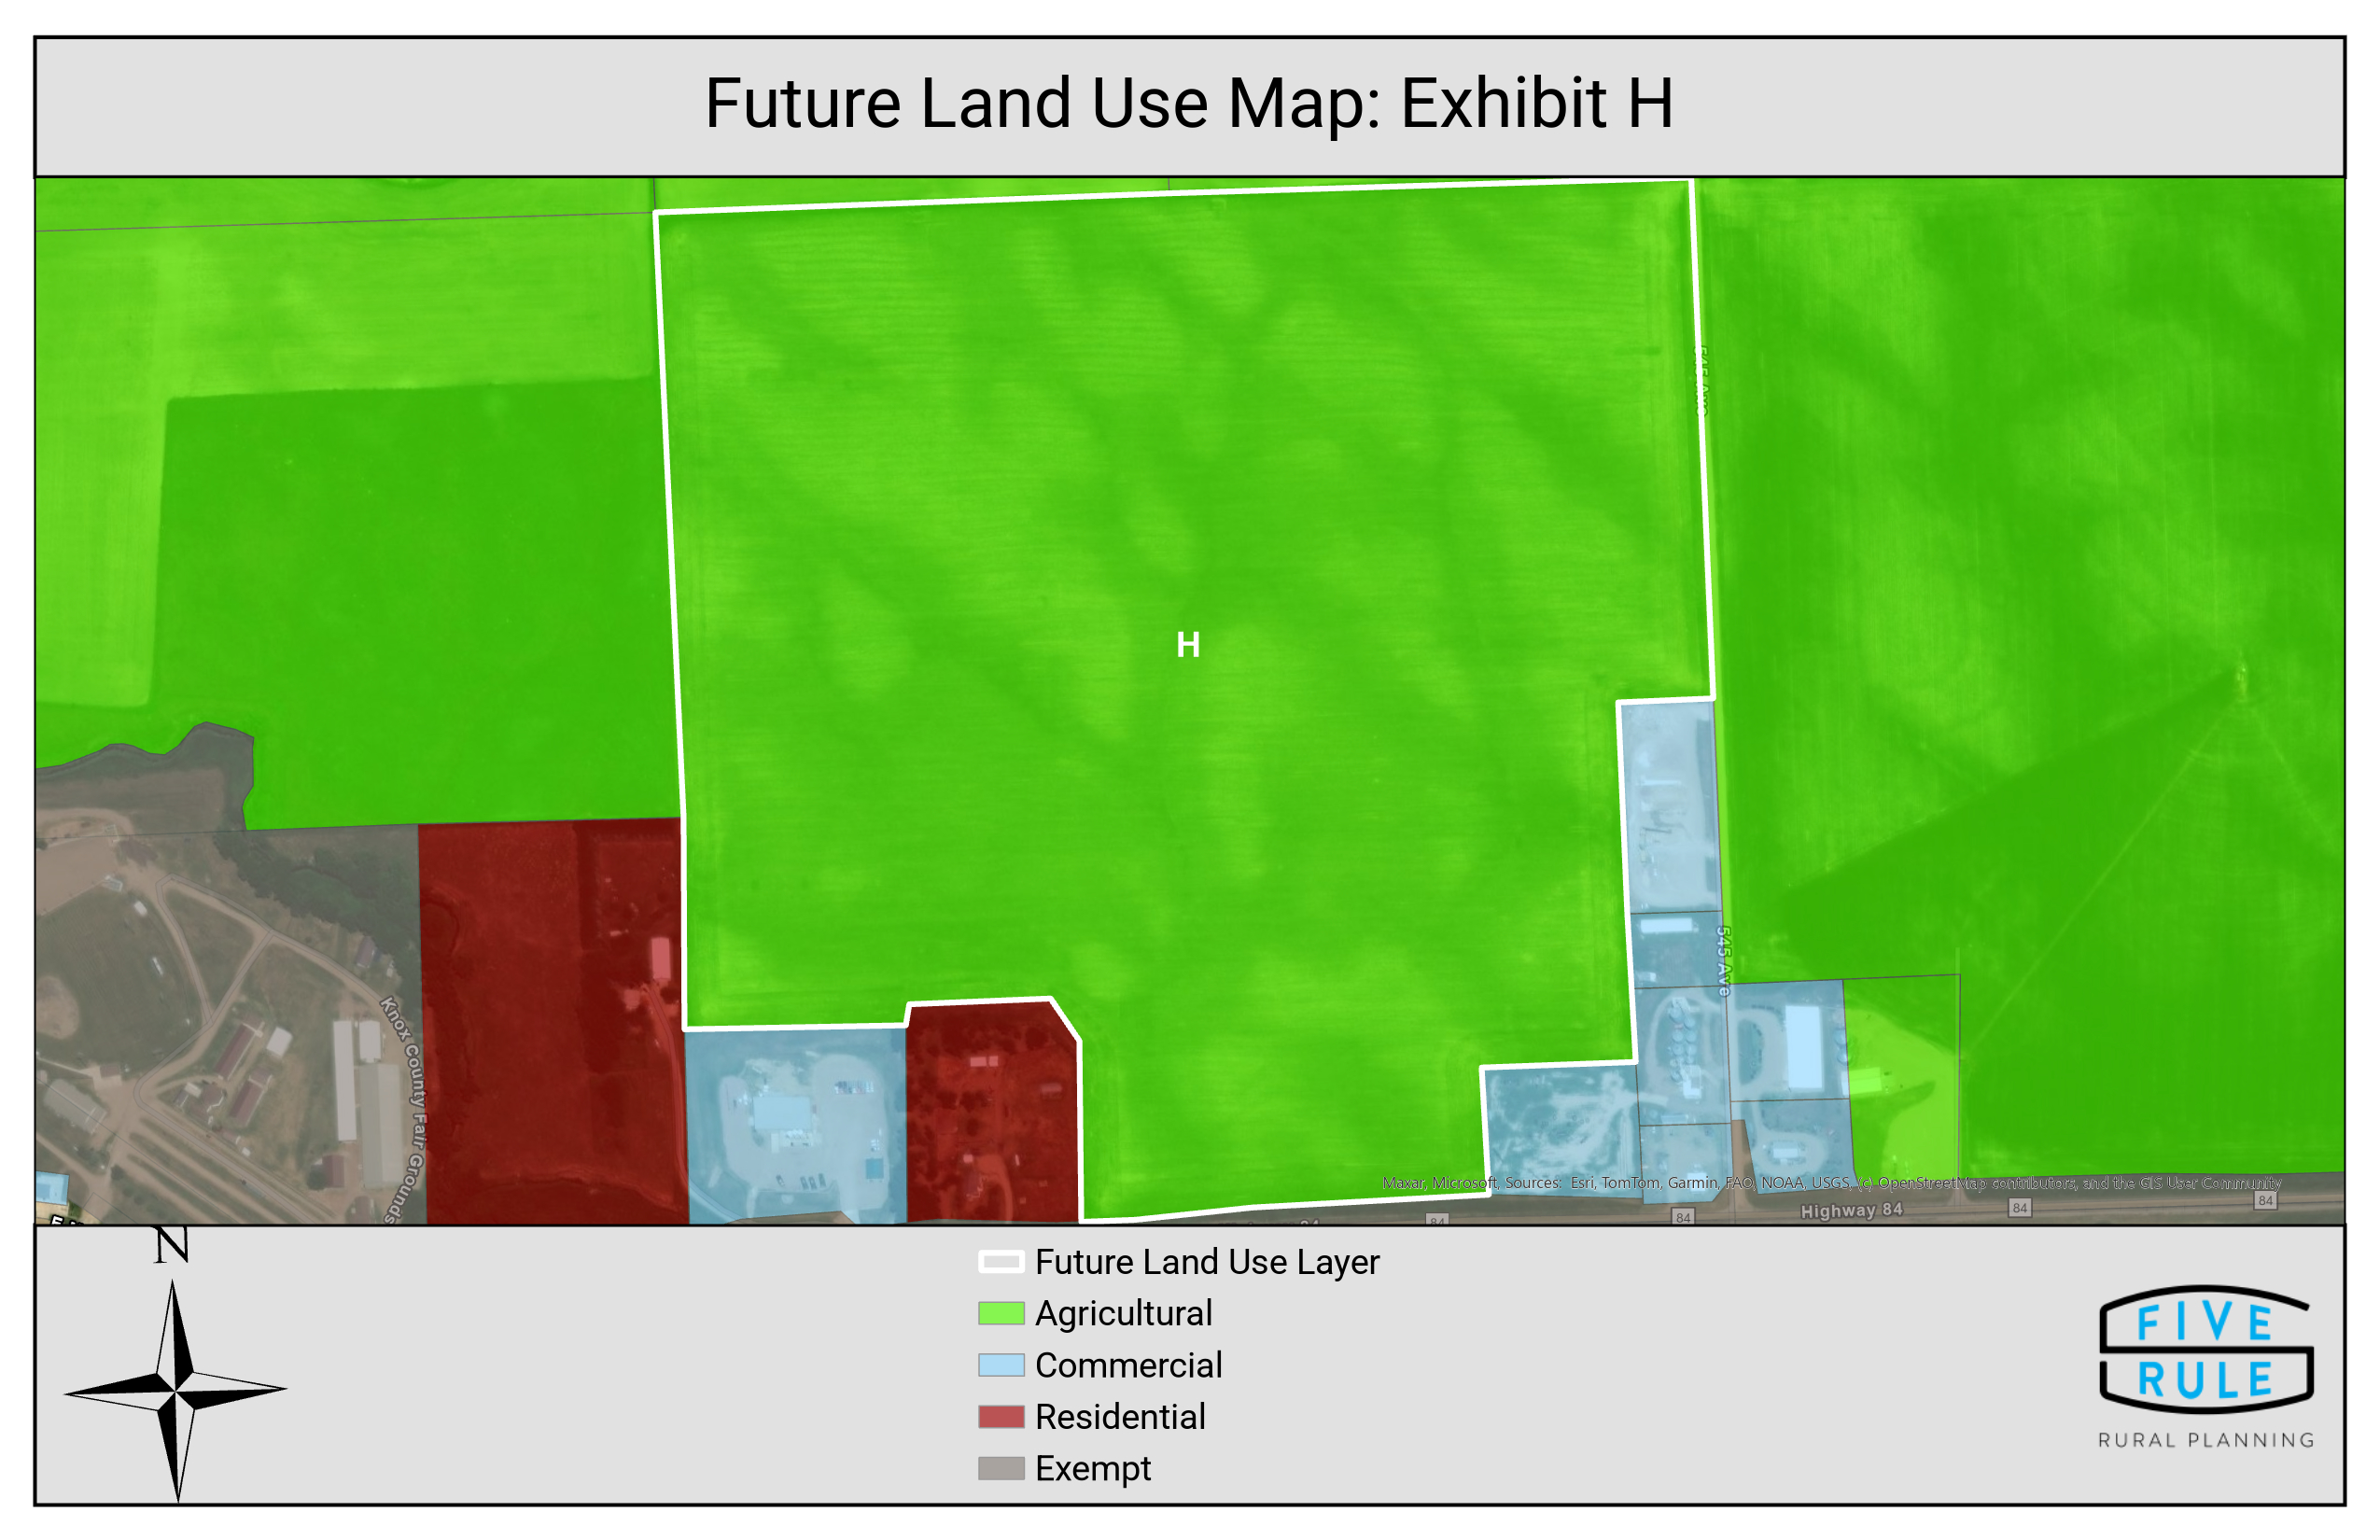
\includepdf[angle = 90]{maps/flu_h.pdf}
\end{landscape}

\pagebreak
\subsection{Description of Future Land Use Exhibits}

\noindent \hl{[i would love to follow up with the Bloomfield folks on this at some point]}

\subsubsection*{Exhibit A}

\noindent Expansion of the Farmers Pride Cooperative, currently listed as commercial land use.

\subsubsection*{Exhibit B}

\noindent Addition of a concessions stand and renovations to softball fields at Robin Schulz Memorial Park.

\subsubsection*{Exhibit C}

\noindent New residential development off of N 1st street, currently listed as residential land use.

\subsubsection*{Exhibit D}

\noindent New residential development east of the Bloomfield Cemetery, currently listed as residential land use.

\subsubsection*{Exhibit E}

\noindent New residential development south of the Dollar General and west of the Good Samaritan Society-Sunset View Assisted Living facility, currently listed as agricultural land use

\subsubsection*{Exhibit F}

\noindent Lands to the west of the swimming pool may be suitable for a new pickleball court or other source of recreation.

\subsubsection*{Exhibit G}

\noindent New residential development along South Broadway street exiting/entering Bloomfield, currently listed as a combination of residential, commercial, and agricultural land use.

\subsubsection*{Exhibit H}

\noindent New expansion of industrial development east of Bloomfield, currently listed as agricultural land use.